\begin{figure}
  \centering
  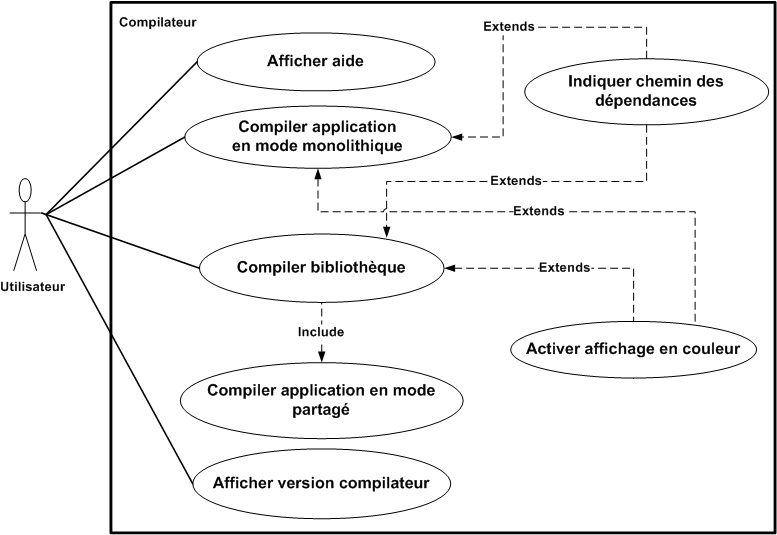
\includegraphics[scale=0.8]{../res/stb/vs_finale_usecase.jpg}
  \caption{\textbf{Cas d'utilisations du compilateur kawa.}}
\end{figure}

%Cas d'utilisation
\subsection{Cas d'utilisation EF\_1}
\fiche
{Afficher l'aide}                    % Nom du cas d'utilisation
{Utilisateur du compilateur}                               % Acteurs concernés
{                                                % Description
  le compilateur affiche 
   la liste des options du compilateur sur la sortie standard à travers une ligne de commande.
}
{
  L'odre de priorité entre le commutateur de help (-h ou --help) et le commutateur de version (-v ou --version) est définit par la première occurrence de l'un des deux commutateur i-e si nous avons un \textbf {-h} avant un \textbf {-v}, le compilateur annule tout le reste et affiche le help 
}                                                % Préconditions
{Commutateur de ligne de commande :kawac -h ou --help}                             % Evénements déclenchants
{Action utilisateur permettant de quiter ce mode }                       % Conditions d'arrêt
% {0.6}{../res/stb/usecase2_flot_event.png}      % Diagramme
{} % acteur(s)
{} % system
{} % flot exceptionsb
 % fin usecase EF_1

\subsection{Cas d'utilisation EF\_2}
\fiche
{Compiler une application en mode monolithique}                    % Nom du cas d'utilisation
{Utilisateur du compilateur}                               % Acteurs concernés
{                                                % Description
  L'utilisateur introduit un ensemble de classes
  kawa afin de les précompiler et de générer le tous dans un seul exécutable.
}
{
	Ensemble de fichiers sources 
	respectant la syntaxe du langage kawa.La non présence des deux commutateurs (-h ou --help) et (-v ou --version) dans la ligne de commande permettant la compilation est obligatoire
}                                                % Préconditions
{Commutateur de ligne de commande :kawac -m filessources.}                             % Evénements déclenchants
{Fin du programme (succès de la compilation),ou bien un message renvoyé par le compialteur indiquant une erreur rencontrée lors de l'analyse de programme, ainsi que dans certains cas le compilateur ne touve pas les fichiers à compiler. 
}                       % Conditions d'arrêt
%{0.6}{../res/stb/usecase2_flot_event.png} 		 % Diagramme
{                                                % Flots d'exceptions
  
}
{} % system
{Abondant provoqué par l'utilisateur, comme la fermeture du terminal au cours de la compilation. } % flot exceptions
% Fin de la fiche du cas d'utilisation 1.


%Cas d'utilisation 2
\subsection{Cas d'utilisation EF\_3}
\fiche
{Compiler une application en mode partagé}                    % Nom du cas d'utilisation
{Utilisateur du compilateur}                               % Acteurs concernés
{                                                % Description
  L’utilisateur introduit un ensemble de sources kawa
 qui peuvent appelés des bibliothèques externes, le compilateur doit être capable de chercher les bibliothèques pour les utiliser ou bien  de les recompiler si nécessaire.La distinction entre ce mode et le mode monolithique c'est l'absence du commutateur -m 
}
{
	Ensemble de fichiers source respectant la syntaxe du langage kawa qui peuvent utiliser des bibliothèques partagées.La non présence des deux commutateurs (-h ou --help) et (-v ou --version) dans la ligne de commande permettant la compilation est obligatoire
	
}                                                % Préconditions
{Commutateur de ligne de commande:kawac filessources [options]}                             % Evénements déclenchants
{Fin du programme (succès de la compilation),ou bien un message renvoyé par le compialteur indiquant une erreur rencontrée lors de l'analyse de programme, ainsi que dans certains cas le compilateur ne touve pas les fichiers à compiler.} % Conditions d'arrêt
%{0.6}{../res/stb/usecase2_flot_event.png} 		 % Diagramme
{                                                % Flots d'exceptions
  
}{} % system
{Abondant provoqué par l'utilisateur,comme la fermeture du terminal au cours de la compilation.} % flot exceptions
% Fin de la fiche du cas d'utilisation 2.


%Cas d'utilisation
\subsection{Cas d'utilisation EF\_4}
\fiche
{Compiler application utilisant des bibliothèques partagées}                      % Nom du cas d'utilisation
{Utilisateur du compilateur}                               % Acteurs concernés
{                                                % Description
    L'utilisateur peut compiler des bibliothèques dynamiques en compilant son application obligatoirement dans un mode partagé,et ceci est possible même si son source n'utilise pas forcément ces bibliothèques externes.      
}
{
  La non présence des deux commutateurs (-h ou --help) et (-v ou --version) dans la ligne de commande permettant la compilation est obligatoire.
}                                                % Préconditions
{Commutateur de ligne de commande:kawac filessources [options] } % Evénements déclenchants
{Fin du programme (succès de la compilation),ou bien un message renvoyé par le compialteur indiquant une erreur rencontrée lors de l'analyse de programme, ainsi que dans certains cas le compilateur ne touve pas les fichiers à compiler.} % Conditions d'arrêt
%{0.6}{../res/stb/usecase3_flot_event.png}     % Diagramme
{                                                % Flots d'exceptions
 
}{} % system
{Abondant provoqué par l'utilisateur,comme la fermeture du terminal au cours de la compilation.} % flot exceptions
% Fin de la fiche du cas d'utilisation 3.
%Cas d'utilisation
\subsection{Cas d'utilisation EF\_5}
\fiche
{Afficher la version du compilateur}                      % Nom du cas d'utilisation
{Utilisateur du compilateur}                               % Acteurs concernés
{                                                % Description
   
L'utilisateur peut savoir la version du compilateur avec le quel compile ses sources et ses bibliothèques  à travers un commutateur de ligne de commande.   
}
{
   L'odre de priorité entre le commutateur de help (-h ou --help) et le commutateur de version (-v ou --version) est définit par la première occurrence de l'un des deux commutateur i-e si nous avons un \textbf {-v} avant un \textbf {-h}, le compilateur annule tout le reste et affiche la version
}                                                % Préconditions
{Commutateur de ligne de commande:kawac -v ou --version}                             % Evénements déclenchants
{Fin du programme.}                       % Conditions d'arrêt
%{0.6}{../res/stb/usecase3_flot_event.png}     % Diagramme
{                                                % Flots d'exceptions
 
}{} % system
{} % flot exceptions
% Fin de la fiche du cas d'utilisation 3.
%Cas d'utilisation
\subsection{Cas d'utilisation EF\_6}
\fiche
{Indiquer les chemins des dépendances entre sources et classes déjà compilées}          % Nom du cas d'utilisation
{Utilisateur du compilateur}                               % Acteurs concernés
{                                                % Description
   
L'utilisateur peut définir les dépendances pour la compilation de son application, en indiquant des chemins entre les sources et des fichiers déjà compilés.}
{
  
}                                                % Préconditions
{Commutateur de ligne de commande:kawac filessources -d path}                             % Evénements déclenchants
{Fin du programme (succès de la compilation),ou bien un message renvoyé par le compialteur indiquant une erreur rencontrée lors de l'analyse de programme, ainsi que dans certains cas le compilateur ne touve pas les fichiers à compiler.}                       % Conditions d'arrêt
%{0.6}{../res/stb/usecase3_flot_event.png}     % Diagramme
{                                                % Flots d'exceptions
 
}{} % condition d'arret
{Abondant provoqué par l'utilisateur, comme la fermeture du terminal au cours de la compilation.} % flot exceptions
% Fin de la fiche du cas d'utilisation 3.

%Cas d'utilisation
\subsection{Cas d'utilisation EF\_7}
\fiche
{Activer l'affichage en couleur}          % Nom du cas d'utilisation
{Utilisateur du compilateur}                               % Acteurs concernés
{                                                % Description
   
  L'utilisateur peut activer l'option de l'affichage en couleur, afin de décorer les messages renvoyés par le compilateur dans les différents modes de compilation.   
}
{
  
}                                                % Préconditions
{Commutateur de ligne de commande:kawac filessource --color}                             % Evénements déclenchants
{Fin du programme.}                       % Conditions d'arrêt
%{0.6}{../res/stb/usecase3_flot_event.png}     % Diagramme
{                                                % Flots d'exceptions
 
}{} % system
{} % flot exceptions
% Fin de la fiche du cas d'utilisation 3.